% !TEX root = ./physics.tex

\chapter{Nature of Light}
	
\section{Introduction}
	
	\subsection{Maxwell's Equations}
	
		Gauss' Law (1813) $\rightarrow$ Electric flux ($\Phi_E = E \times \Delta A$) of any closed surface.

		Electric flux is defined as the electric field (E) times the component of the area perpendicular to the field.

		The area integral of the electric field over any closed surface is equal to the net charge divided by the permittivity of free space.

		Gauss' Law of Magnetism

		The net magnetic flux out of any enclosed surface is zero

		For any magnetic dipole, any magnetic flux directed inward toward the south pole will equal the flux outward from the north pole

		There are no magnetic monopoles

		Ampere's Law (1826)

		Describes the magnetic field around a closed conductor loop to the strength of the electric current flowing through the loop

		A changing magnetic field creates a changing electric field
		A changing electric field creates a changing magnetic field

		This means that they can like propagate each other


		Hertz's Experiment

		Maxwell predicted there would be other forms of electromagnetic waves - that light was just one example

\newpage

\section{Practical Investigation - Estimating the speed of light}

	\subsection{Introduction}
	
		Using the equation $v = f \lambda$ to determine the speed of light

		The microwave is designed such that microwaves are reflected off the opposite wall to create a standing wave. This causes fluctuations in energy depending on the point of the wave (at the maximums). The wavelength can be determined by measuring the distance between each gap in the chocolate.

		Accuracy can be improved by minimising size of holes. The size of the microwaves is small, so larger holes will create significant error

	\textbf{Aim}: To estimate the speed of light

	\subsection{Materials}
	
		\begin{itemize}
			\item Large chocolate block
			\item Microwave (frequency of 2450 MHz)
		\end{itemize}

	\subsection{Risk Assessment}
		\begin{table}[H]
			\centering
			\begin{tabular}{p{7cm}|p{7cm}}
				Hazard & Precaution \\ \hline
				Burning from hot chocolate & Wear oven mitts when removing the chocolate and allow adequate cooling before handling \\
				Dropping parts of the microwave & Handle the baseplate of the microwave with caution
			\end{tabular}
		\end{table}

	\subsection{Method}
	
		\begin{enumerate}
			\item Prepare a 
		\end{enumerate}

\section{Spectroscopy} \label{08/05/2025}
	
	\subsection{Star Analysis}
	
		The qualities of stars can be predicted by observing their colours. Different temperatures emit different levels of visible light

\newpage

\section{Analysis of Star Spectra}

	\subsection{}

	A star's inner nucleus produces a light source that contains a continuous spectrum of all wavelengths, with a peak at a certain point depending on the temperature of the star.

	Stars are made of a ball of gas that varies the colour emitted by the star as a whole. This is due to fluctuation in energy levels of atoms, exciting electrons within these atoms and allowing electrons to "jump" to another orbital level. The electrons in the excited state absorb specific wavelengths of light, and create gaps in the light spectrum after passing through the gas.

	The excited electrons will also fall, emitting energy and also providing information about the star. Hence, the composition profile of the star's gas can be determined using it's emission spectrum (with peaks) or it's absorption spectrum (with dips in the full spectrum).

	\subsection{Spectroscope}
	
		A spectroscope is a device used to display the absorption spectrum of a given element

		High voltage is passed through a tube containing a particular element. The light emitted by the gas is passed through a prism to separate the wavelengths and projected onto a screen. This can be used to analysis the chemical composition of the star, as well as other physical properties.

		\subsubsection{Analysis of the Absorption Spectrum}
		
			\begin{itemize}
				\item Rotational velocity
					\begin{itemize}
						\item As the star rotates, the light is blue or red shifted. This creates wider lines on the absorption spectrum as the rotational velocity increases
					\end{itemize}

				\item Translational velocity
					\begin{itemize}
						\item Due to movement towards and away from a fixed point, the entire light spectrum can either be blue or red shifted
						\item All the lines on the spectrum are shifted equally depending on the relative velocity of the star
						\item By using the known properties of elements (commonly hydrogen), the spectrum can be compared to that of one where the star was not moving
					\end{itemize}

				\item Density
					\begin{itemize}
						\item If the star is made of high density gas, more collisions occur between the atoms and further the electrons
						\item These collisions vary the energy that the electron has as it moves between orbital states, creating small variations of wavelength produced
						\item This variation is depicted on the spectrum as a blurred line
					\end{itemize}
				
				\item Chemical composition
					\begin{itemize}
						\item Different chemicals produce different emissions spectra
						\item A star will emit multiple overlapping spectra that form the spectrum that is visible from an external observer
					\end{itemize}
			\end{itemize}

\section{Diffraction and Interference} \label{15/05/2025}
	
	Diffraction is the spreading out of a waves when it passes a barrier or small opening. The size of the obstacle should be the same order of magnitude as the wavelength.

	Interference occurs when two waves reach a point at the same time, causing the waves to combine either constructively or destructively

	Chromatic light contains many wavelengths of light, however interference can only be observed when the light is monochromatic and in phase. The best way to achieve this is by a laser.

	\subsection{Young's Double Slit Experiment}
	
		In order for the two-slit interference pattern to result, the light hitting the double slit should be monochromatic and coherent. $d$ is the separation of the double slits, $S_{2}M - S_{1}M$ is the path difference, $L$ is the distance between the double slits to the screen, and $x$ is the distance from the central maximum to position $M$.

		The central maximum is always a bright fringe.

		The first minimum is produced when the wave from $S_1$ has travelled one half of a wavelength further than the save from $S_2$. When $S_1 C - S_2 C = \lambda$, the area is brighter.

		\begin{figure}[H]
			\centering
			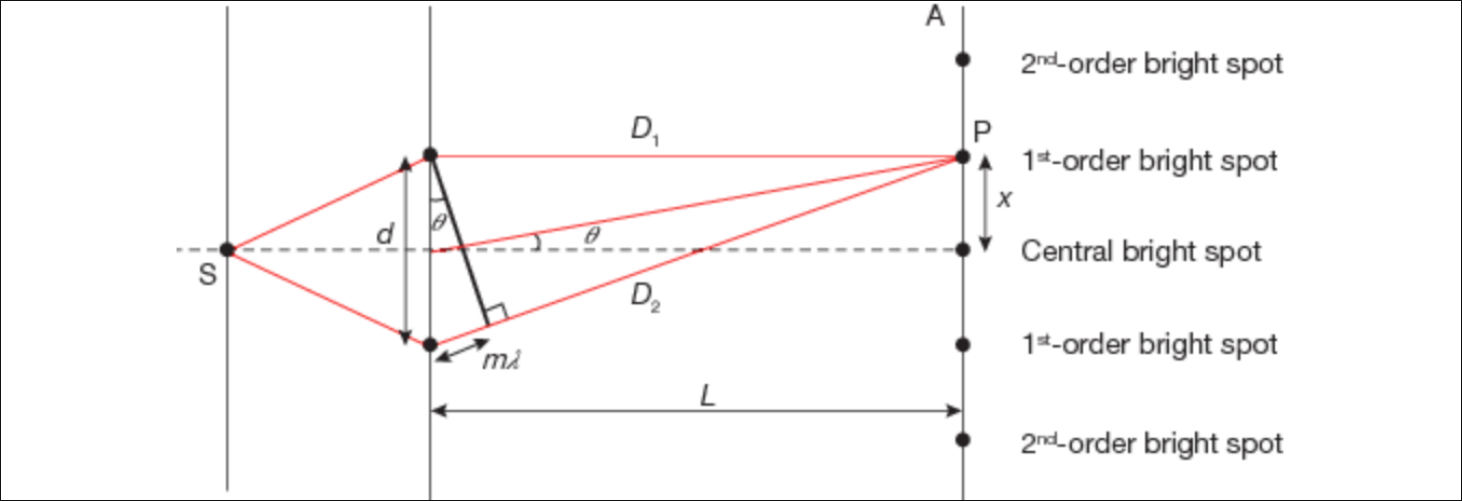
\includegraphics[width=15cm]{young_double_slit.png}
		\end{figure}

\section{Light: Wave or Particle} \label{20/05/2025}

	\subsection{Newton's Particle Model}
		
		\begin{itemize}
			\item Light consists of small particles
			\item These particles have mass and obey the laws of physics (advanced mechanics)
			\item The particles are so small that when two beams cross they don't collide or interact
			\item Once ejected from a light source, the particles continue in a straight line
			\item Light would cast shadows
			\item Limitation: light was not affected by gravity like it should be
		\end{itemize}
	
	\subsection{Huygen's Wave Model}
	
		\begin{itemize}
			\item Each point on a wavefront behaves as a point source for wavelets in the direction of propagation (longitudinal)
			\item 
		\end{itemize}

\section{Quantum Light}

	As temperature increases, the energy emitted and frequency increases

	The peak wavelength is related to the temperature of the blackbody
	
	Wien's Law states that $\lambda _{max} = \frac{b}{T}$ where $\lambda _{max}$ is peak wavelength, $T$ is the temperature of the surface of the body (in kelvin) and $b$ is Wien's constant (provided on datasheet)

	The wave model of light predicts that as the wavelength increases, the intensity of light should increase. At low wavelengths, the intensity should reach infinity. The classical wave model cannot explain the black body radiation curve.

	To explain the blackbody radiation curve, Max Planck made two assumptions:

		\begin{itemize}
			\item The energy of the oscillators was quantized (whole number) - one quantum of energy possesses just one wavelength
			\item The energy of each of the packets is calculated by using $E = n\hbar f$
		\end{itemize}

	Thermal energy comes in packets called quanta.

	\subsection{Photoelectric effect}
	
		JJ Thomson established that UV light caused electrons to be emitted from a sheet of metal.

		Electrons will absorb UV light, providing enough energy to liberate valence electrons. This creates a photoelectric current.

		Lenard Experiment (photoelectric)
		
		He found that a current can be produced and measured when the electrons emitted by radiation strikes a collector

		The most energetic electrons can overcome the applied voltage (stopping voltage)

		Increasing light intensity will increasing the current, however will not change the stopping voltage

		Increasing the frequency of the light will produce a constant photocurrent, but will change the stopping voltage.

	\subsection{Faults of the Wave Model}
	
		The photoelectric effect happens instantly. The wave model states that energy would build up to release electrons, however this is not true. The radiation of lower frequency light will determine its stopping voltage. If the light does cause the emission of photoelectrons, increasing the intensity of the light will increase the number of photoelectrons emitted per second.
\newpage

	\subsection{Practical Investigation}

		Effect of intensity on photoelectrons
	
		\begin{table}[H]
			\centering
			\begin{tabular}{p{7cm}|p{7cm}}
				\textbf{Diameter of aperture (cm)}	& \textbf{Photocurrent (nA)}	\\ \hline
				0.7					& 96.4				\\
				1					& 197				\\
				1.4					& 270				\\
				2					& 340				\\

			\end{tabular}
		\end{table}
		
		Effect of light frequency + max KE of photoelectrons
		\begin{table}[H]
			\centering
			\begin{tabular}{p{2cm}|p{3.5cm}|p{3.5cm}|p{4cm}}
				\textbf{Colour}	& \textbf{Wavelength (nm)}	& \textbf{Frequency (Hz)}	& \textbf{Stopping voltage (V)} \\ \hline
				Blue		& 432				& 				& -0.771			\\
				Green		& 471				& 				& -0.616			\\
				Yellow		& 501				& 				& -0.506			\\
				Red		& 582 				& 				& -0.237			\\
			\end{tabular}
		\end{table}

\section{Einstein's Explanation of the Photoelectric Effect}

	\begin{itemize}
		\item Light behaves like a stream of particles carrying energy given by Planck's equation ($E = \hbar f$)
		\item The energy of the light particle (photon)is related to its wavelength ($E = hc/f$)
		\item The intensity of the beam of light is determined not by the amplitude but by the number of photons that pass through a unit area * photon energy
		\item All of the energy of one photon is absorbed by only one electron
	\end{itemize}

\section{Principle of Relativity}

	Constancy of speed of light

	James Maxwell has shown that the speed of light is constant ($c = \frac{1}{\sqrt{\mu_0 \epsilon _0}}$)

	If the speed of light is absolute, then there is no absolute (universally valid) frame of reference.

	Consider a person standing next to a moving car. The light from the headlights are therefore perceived as $v = c + v_c$, where the velocity of the car is $v_c$. This is not the case.

	If $c$ is constant, than classical relative time and distance is not accurate. Hence the definition of the metre and second were adapted relative to the absolute speed of light.

	\subsection{Einstein's Postulates}
	
		\begin{itemize}
			\item Light was already established as an electromagnetic wave
			\item The aether was believed to be a medium through which electromagnetic waves were transmitted and that all matter moved relative to the aether. As it is always stationary, it is considered as an absolute frame of reference. This contradicts Einstein's postulate that all inertial frames of reference are equivalent and that there is no absolute FOR.
			\item The Michelson-Morley experiment involved using mirrors to compare the speed of light travelling parallel and perpendicular to the aether wind (the relative motion to the aether)
				\begin{itemize}
					\item When the light reflected off the mirror and went against the aether wind, a difference in the speed of light was expected.
					\item The experiment found that there was no change in velocity, hence either the aether doesn't exist, or it doesn't affect the speed of light
					\item Hence, confirming the Michelson-Morley experiment.
				\end{itemize}
		\end{itemize}

		Prior to Einstein's postulates, time and space were viewed as absolute. Speed of light is constant, therefore time and space cannot be defined absolutely. Consequently, time dilation and length contraction occurs.

	\subsection{Time Dilation}
	
		Consider a light clock that consists of two mirrors and a beam of light bouncing between them.

		\begin{align*}
			v &= \frac{d}{t} \\
			\Delta t_0 = \frac{2d}{c}
		\end{align*}
	
\section{Observing Special Relativity}

	\subsubsection{Muon Decay}
	
		Muons are fundamental particles similar to electrons but with a smaller mass. This means they only have a half life of 2.2 microseconds and are able to travel at above 0.99 times the speed of light. Since the muons move very quickly, they experience time dilation that reduces the rate of decay and allows nearly 25\% of the muons to reach Earth.

	\subsubsection{Atomic Clocks}
	
		An atomic clock on the ground an on a plane experience different velocities and the accuracy of the clocks allows the extent of the time dilation to be measured.

	\subsubsection{GPS Satellites}
	
		All GPS satellites must account for time dilation because electromagnetic waves travelling at the speed of light will travel an extra metre in 3 nanoseconds.

	\subsubsection{Particle Accelerators}
	
		The momentum of particles inside the loop of a particle accelerator must be careful controlled.

	\subsubsection{Cosmological Studies}
	
		The sun creates energy by combining hydrogen to form helium.

		\begin{align*}
			E = mc^2
		\end{align*}

\section{Relativistic Momentum} \label{26/06/2025}

	\begin{itemize}
		\item If $F=ma$, then why can't an object be accelerated to $c$
		\item When $F$ increases, momentum also increases hence impulse is experienced
		\item Mass is never affected by velocity
		\item The rate of motion is affected by time dilation.
	\end{itemize}

	\begin{align*}
		\Delta p = \gamma m v
	\end{align*}

	The mass that is missing is mass defect, released as energy.
